\documentclass{article}

\usepackage{Sweave}
\begin{document}
\Sconcordance{concordance:prief_outline.tex:prief_outline.Rnw:%
1 2 1 1 0 47 1}


\begin{figure}[h!]
  \centering
 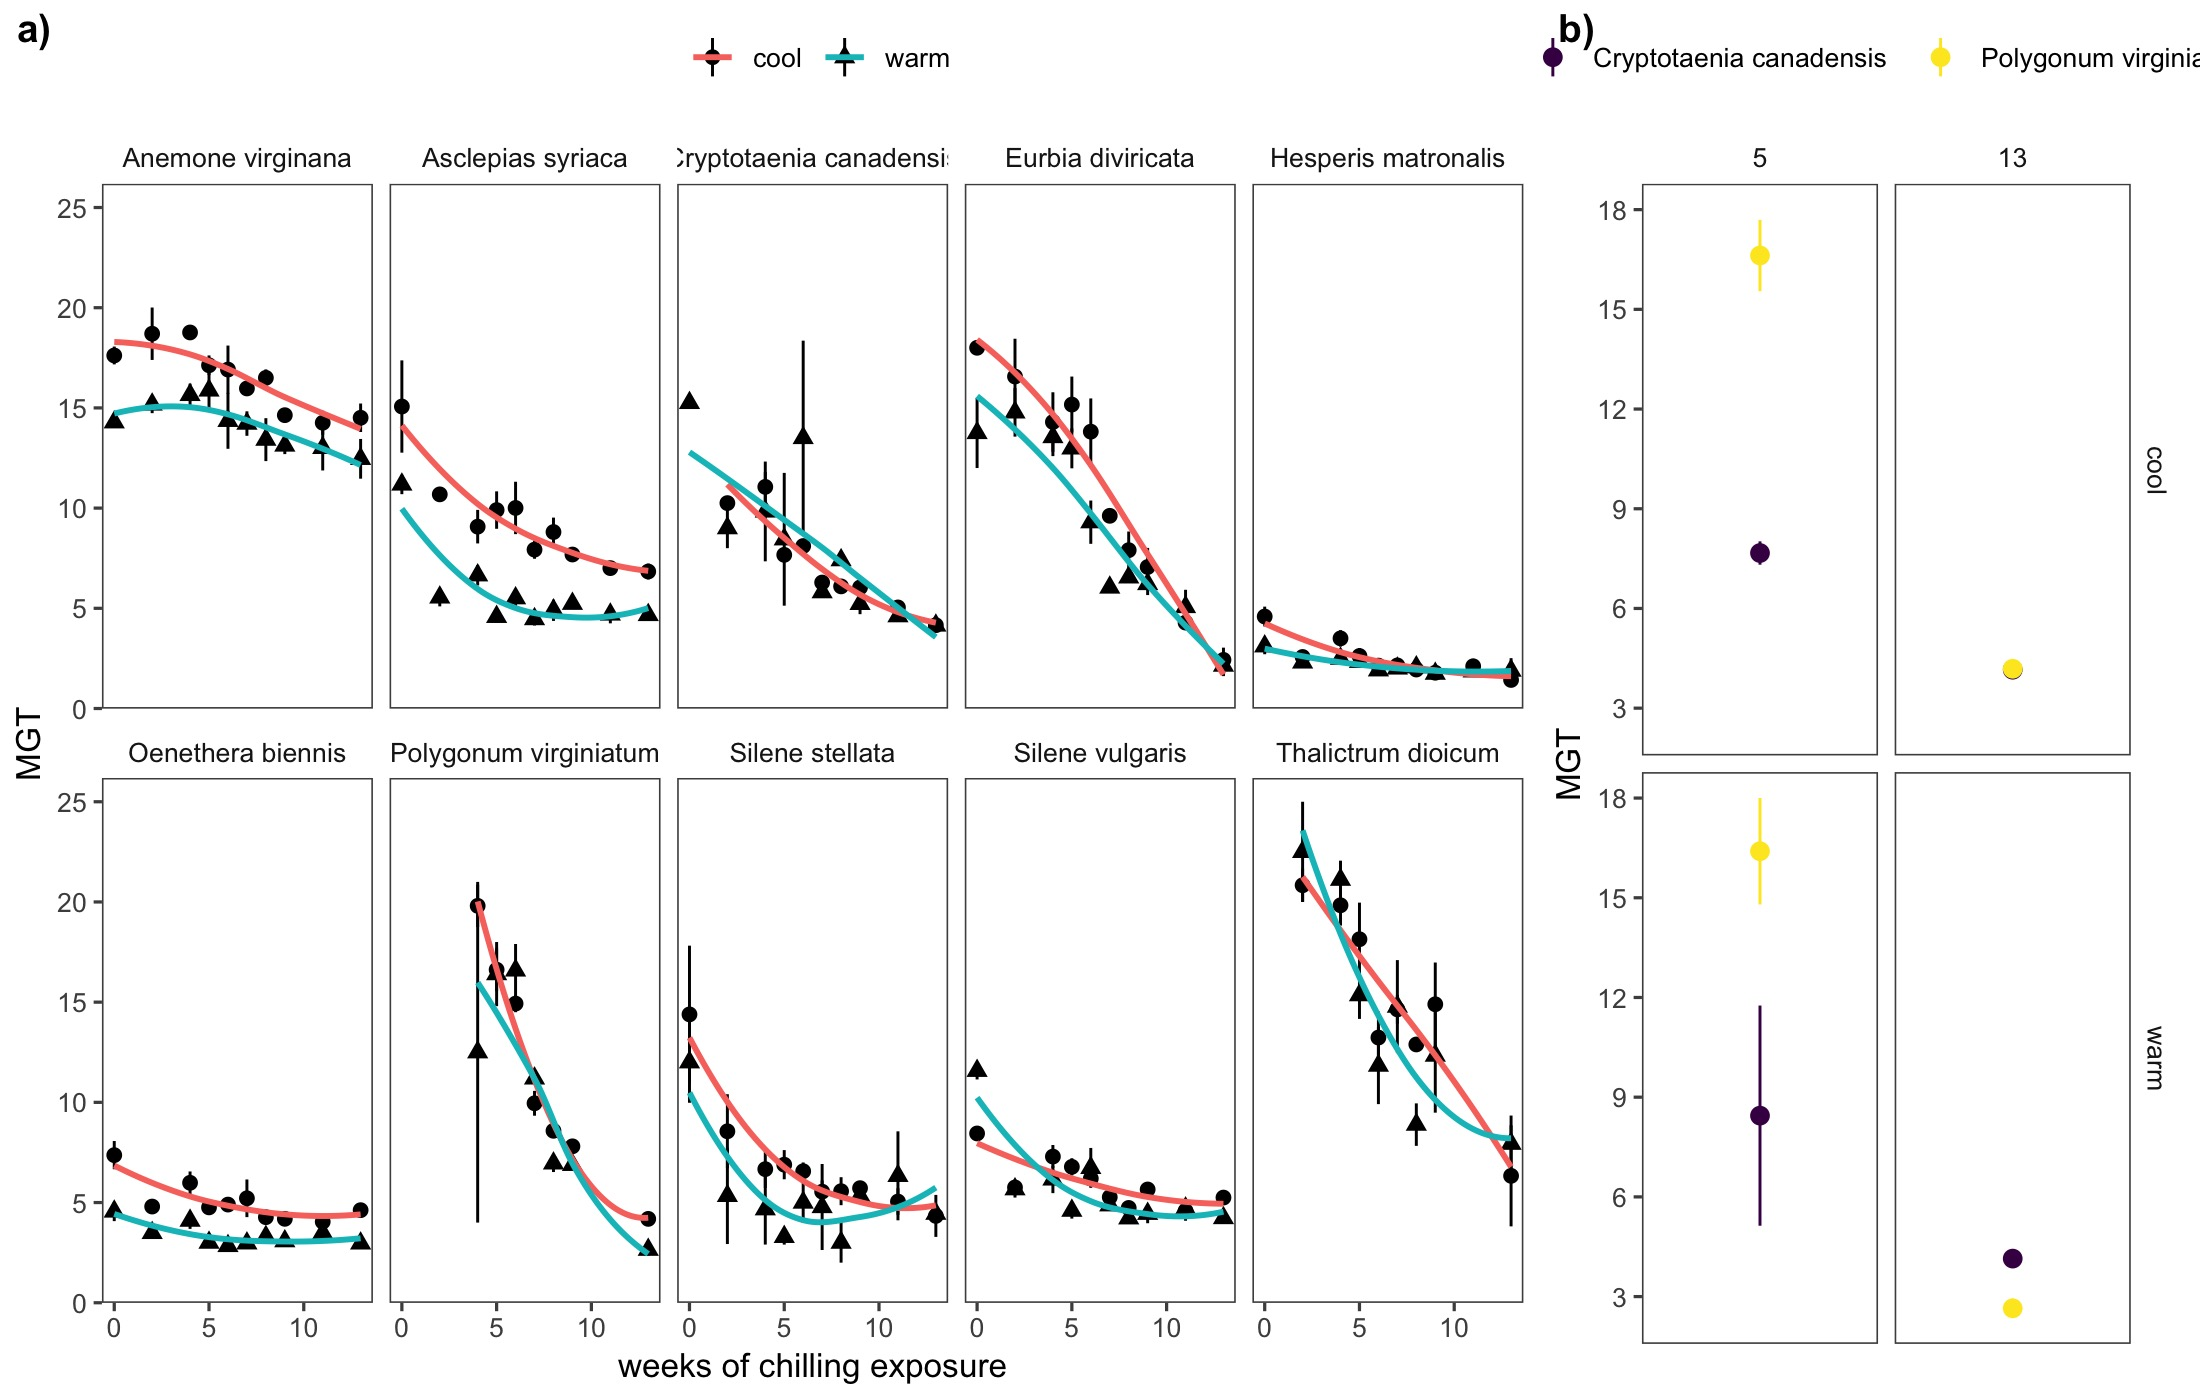
\includegraphics[width=\textwidth]{..//plots/empricalplots2.jpeg}
    \caption{potential empirical plot style?}
    \label{Fig:emp}
\end{figure}

\begin{figure}[h!]
  \centering
 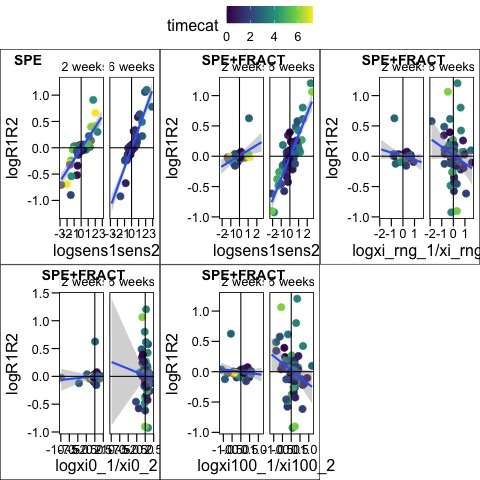
\includegraphics[width=\textwidth]{..//plots/coexistance_runner.jpeg}
    \caption{4\% of high chill cases result in coexistence and 3\% of low chill cases. The slope gets steeper in low chill scenario. Overall pretty limited change to coexistence overall, you just need more exteme differences in sensitivity to acheive it. Does this mean we need to tune the parameters?}
    \label{Fig:coexistence}
\end{figure}


\begin{figure}[h!]
  \centering
 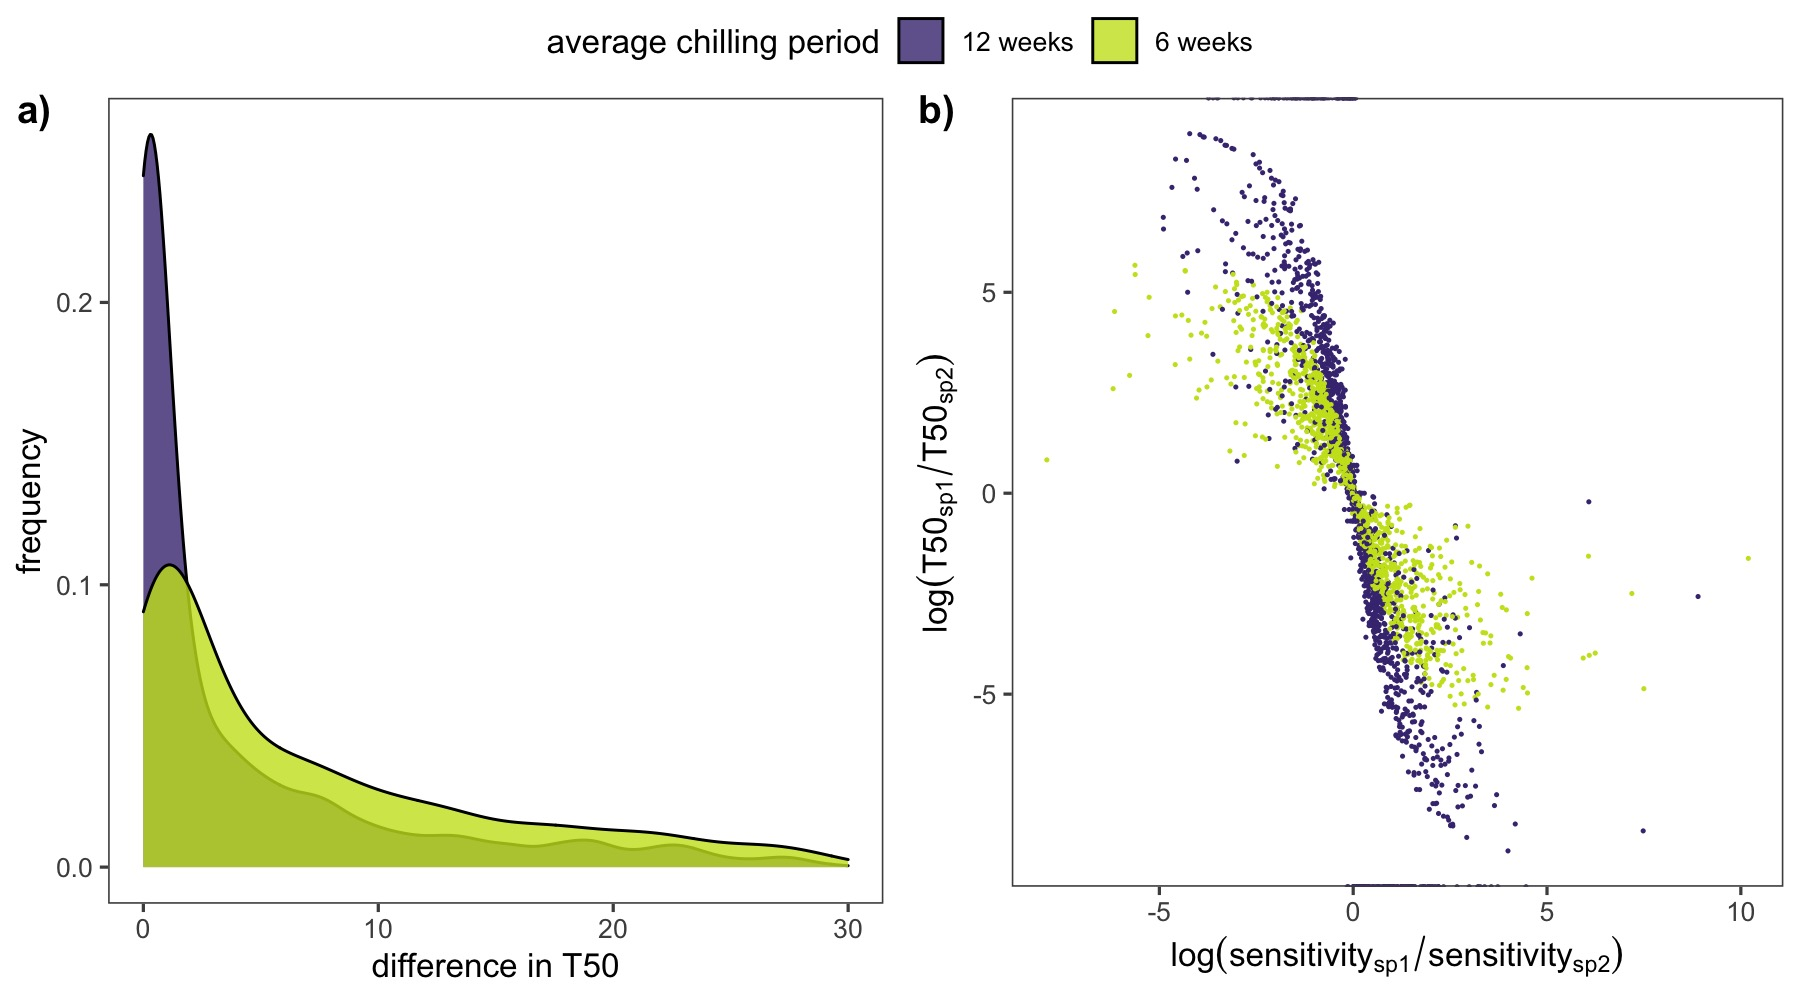
\includegraphics[width=\textwidth]{..//plots/coexistance_chilldiffs.jpeg}
    \caption{The mean difference in germination is lower with high chill (a). The same differences in sensitivity manifest in larger differences in germination time under high chill, so smaller differences in sensisitivity are more likely to lead to coexistence}
    \label{Fig:differences}
\end{figure}

\begin{figure}[h!]
  \centering
 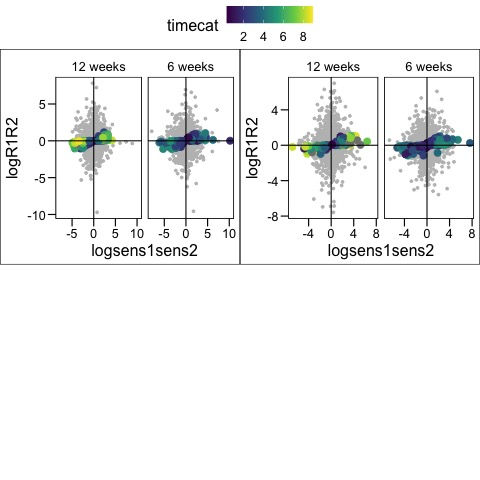
\includegraphics[width=\textwidth]{..//plots/dominance.jpeg}
    \caption{Not sure if we want to go down this path, but I also looked at scenarios where the worse competitor wins due to priority effects. This becomes more common in lower chilling world (180 cases vs 110 cases or 12\% of cases of competitive exclusion vs. 7\%). Suggesting (maybe) SPE's will play a strong role in compeition under warming?}
    \label{Fig:differences}
\end{figure}

\end{document}
